\documentclass[a4paper,12pt]{article} % тип документа

%  Русский язык
\usepackage[T2A]{fontenc}			% кодировка
\usepackage[utf8]{inputenc}			% кодировка исходного текста
\usepackage[english,russian]{babel}	% локализация и переносы

\usepackage{graphicx, scalerel}               % импорт изображений
\usepackage{wrapfig}                % обтекаемые изображения
\graphicspath{{pictures/}}          % обращение к подкаталогу с изображениями
\usepackage[14pt]{extsizes}         % для того чтобы задать нестандартный 14-ый размер шрифта
\usepackage[warn]{mathtext}         % русский язык в формулах
\usepackage{indentfirst}            % indent first
\usepackage[margin = 25mm]{geometry}% отступы полей
\usepackage[table,xcdraw]{xcolor}   % таблицы
\usepackage{amsmath,amsfonts,amssymb,amsthm,mathtools} % Математика
\usepackage{wasysym}                % ???
\usepackage{upgreek}                % ???  
\usepackage{caption}
\usepackage{multirow}
\captionsetup{labelsep=period}
\usepackage[font=small,labelfont=bf]{caption}
\usepackage{gensymb} % degree symbol
\usepackage{tikz}
\usetikzlibrary{positioning}


\begin{document}
	
	
	\begin{center}
		
		\textbf{НАЦИОНАЛЬНЫЙ ИССЛЕДОВАТЕЛЬСКИЙ УНИВЕРСИТЕТ \\ <<МОСКОВСКИЙ ФИЗИКО-ТЕХНИЧЕСКИЙ ИНСТИТУТ>>}
		\vspace{13ex}
		
		\textbf{Лабораторная работа 4.7.3\\ <<Изучение поляризованного света>>}
		\vspace{40ex}
		
		\normalsize{Шумаков Иван Игоревич \\ студент группы Б01-009\\ 3 курс ФРКТ\\}
	\end{center}
	
	\vfill 
	
	\begin{center}
		г. Долгопрудный\\ 
		2022 г.
	\end{center}
	
	
	\thispagestyle{empty} % выключаем отображение номера для этой страницы
	\newpage


    \textbf{Цель работы:} Измерить пробег $\alpha$-частицы в воздухе двумя разными способами.\par
    \textbf{В работе используются:} барометр, сцинтилляционный счетчик, ионизационная камера.\par
    
    
    \section{Теоретические сведения}

        В качестве источника альфа-частиц используется $ ^{239}  $Pu  с периодом полураспада $ T_{1/2} = 2,44 \cdot 10^4 $ лет.
        Альфа-частицы, испускаемые $ ^{239} Pu $, состоят из трех моноэнергетических групп, различие между которыми лежит в пределах 50 кэВ.
        При той точности, которая достигается в наших опытах, их можно считать совпадающими по энергии, равной 5,15 МэВ.\par
        При $\alpha$-распаде исходное родительское ядро испускает ядро гелия и превращается в дочернее ядро, число протонов и число протонов уменьшается на две единицы.
        Функциональная свзяь между энергией $\alpha$-частицы $E$ и периодом полураспада радиоактивного ядра $T_{1/2}$ хорошо описывается формулой:
        \begin{equation}
            \lg T_{1/2} = \frac{a}{\sqrt{E}} + b.
        \end{equation}\par
        Экспоненциальный характер этого процесса возникает вследствие экспоненциального затухания волновой функции в области под барьером, где потенциальная энергия больше энергии частицы.\par
        Экспериментально энергию $\alpha$-частиц удобно определять по величине их пробега в веществе.
        Энергия частицы теряется в следствии ионизации частиц среды. 
        В следствии этого появляется свободные носители заряда, которые можно измерить.\par
        Для описания связи между энергией $\alpha$-частицы и ее пробегом пользуются эмпирическими соотношениями. 
        В диапазоне энергий $\alpha$-частиц от 4 до 9 МэВ эта связь хорошо описывается выражением:
        \begin{equation}
            R = 0,32E^{3/2}
        \end{equation}\par
        В этой формуле пробег $\alpha$-частиц в воздухе R (при $15 ^oC$ и нормальном атмосферном давлении) выражается в сантиметрах, а энергия E — в мегаэлектрон-вольтах.
    \newpage

    \section{Ионизационная камера}
        
        \subsection{Экспериментальная установка}    

            \begin{figure}[h]
                \centering
                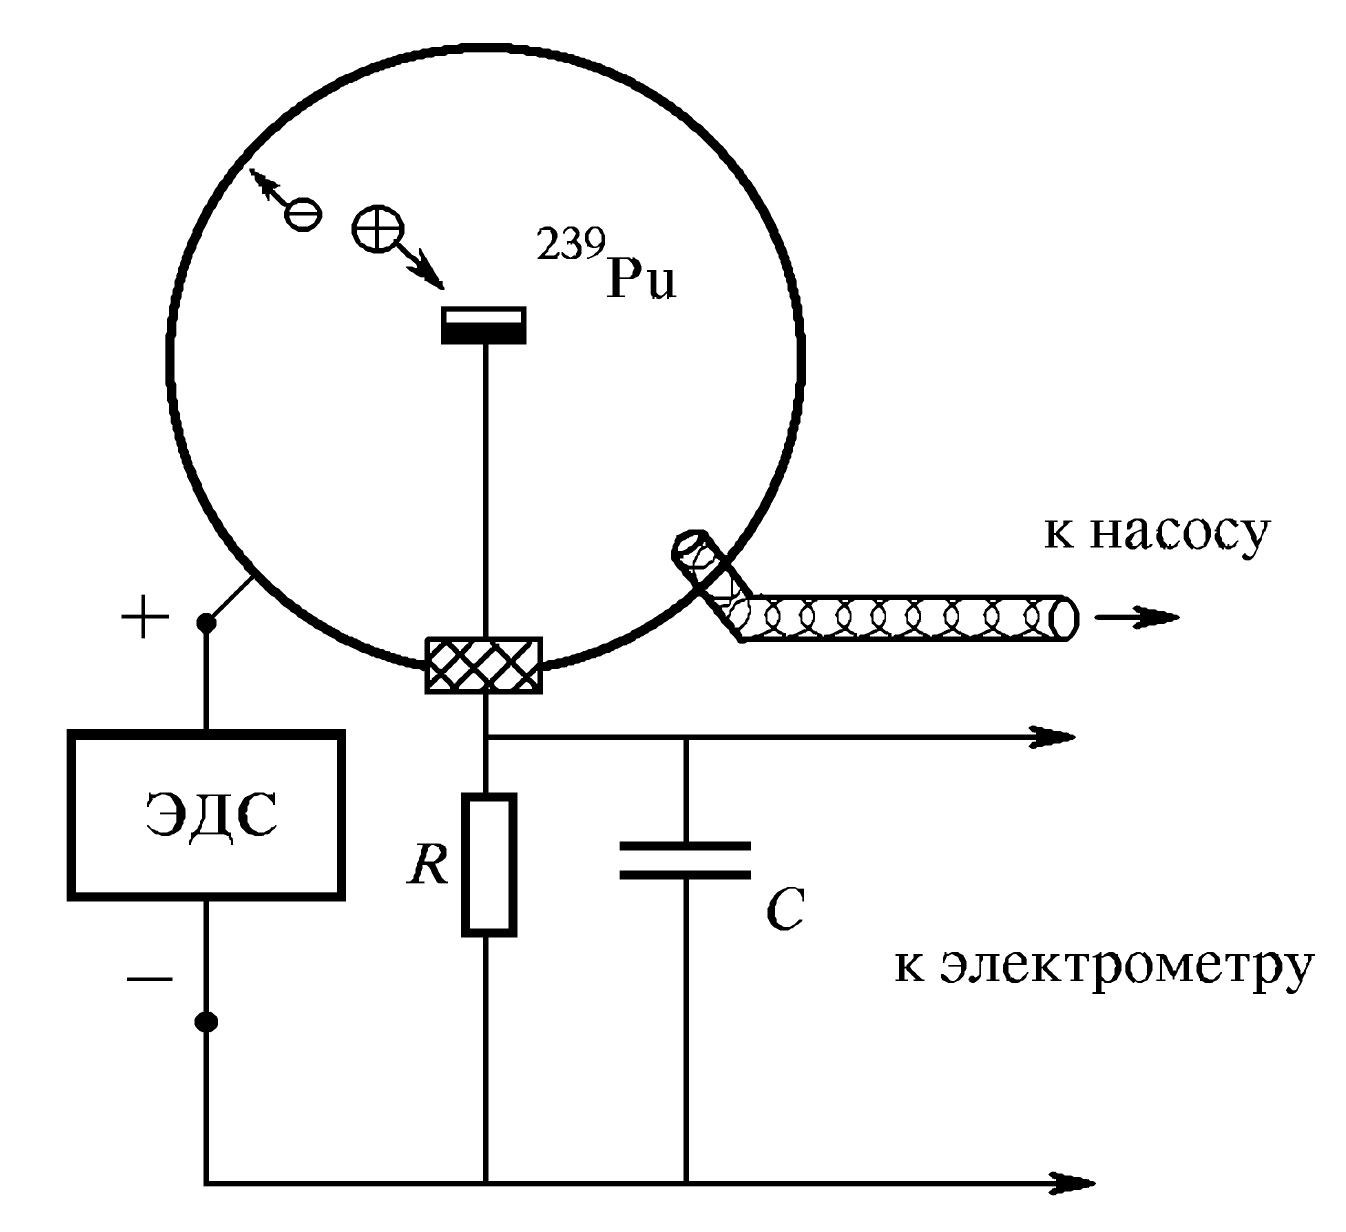
\includegraphics[width=11cm]{img/Ion.PNG}
                \caption{Схема экспериментальной установки}
                \label{fig1}
            \end{figure}
            Ионизационная камера — прибор для количественного измерения ионизации, произведенной заряженными частицами при прохождении через газ.
            Камера представляет собой наполненный газом сосуд с двумя электродами. 
            Сферическая стенка прибора служит одним из электродов, второй электрод вводится в газ через изолирующую пробку.
            К электродам подводится постоянное напряжение от источника ЭДС.\par

        \subsection{Ход работы}

            В данном эксперименте была получена зависимость давления в камере от тока, протекающего через схему.
            Результаты представлены в таблице.\par
            По полученным данным была определена точка перегиба. 
            Ей соответствует состояние камеры, когда $\alpha$-частицы полностью теряют энергию вследствии ионизации.
            Таким образом, зная диаметр камеры можно оперделить длину свободного пробега $\alpha$-частицы.\par
            \begin{table}[h!]
                \centering
                \begin{tabular}{|c|c|c|c|}
                \hline
                $\Delta P [\text{мм.рт.ст}]$& I [\text{пкА}] & $\Delta P [\text{мм.рт.ст}]$ & I [\text{пкА}] \\ \hline
                720      & 9   & 370      & 611 \\ \hline
                710      & 25  & 350      & 652 \\ \hline
                680      & 70  & 330      & 695 \\ \hline
                660      & 102 & 310      & 735 \\ \hline
                640      & 132 & 290      & 780 \\ \hline
                620      & 165 & 260      & 845 \\ \hline
                600      & 202 & 230      & 900 \\ \hline
                570      & 249 & 200      & 930 \\ \hline
                540      & 300 & 180      & 940 \\ \hline
                510      & 346 & 160      & 940 \\ \hline
                480      & 404 & 140      & 935 \\ \hline
                470      & 429 & 120      & 935 \\ \hline
                450      & 456 & 100      & 930 \\ \hline
                430      & 494 & 80       & 925 \\ \hline
                410      & 534 & 50       & 915 \\ \hline
                390      & 576 & 30       & 910 \\ \hline
                \end{tabular}
            \end{table} 
            По экспериментальным данным был построен график I(P). 
            На нем было выделено 2 группы точек: зона роста ионного тока и зона плато. 
            Каждая из них была аппроксимирована прямой. 
            Пересечению этих прямых соответствует точка перегиба.\par
            \begin{figure}[h!]
                \centering
                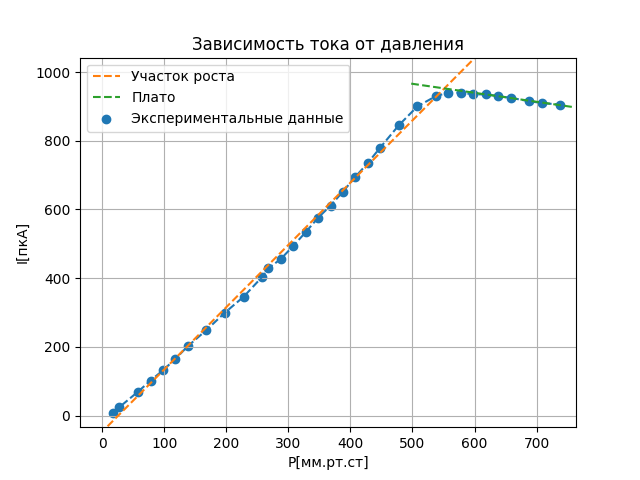
\includegraphics[width=18cm]{img/Graph1.PNG}
                \caption{График зависимоти I(P)}
                \label{graph1}
            \end{figure}
    \newpage

            Исходя из графика точка перегиба имеет координаты:
            \begin{equation}
                P = 550 [\text{мм.рт.ст.}] \hspace{10mm}
                I = 952 [\text{пкА}]
            \end{equation}\par        
            Погрешности коэффициентов каждого из графиков примерно равны одному проценту.
            Поскольку точка перегиба находится из экстреполяции реальных значений, примем погрешность метода равной отношению отклониения экстраполяции от реальных данных к значению в точке.\par
            Таким образом примем относительную погрешность точки перегиба, как:
            \begin{equation}
                \delta \approx \delta_k + \delta_{method} \approx 0.01 + \frac{20}{950} \approx 0.04 
            \end{equation}\par
            Окончательное значение точки перегиба:
            \begin{equation}
                P_o = 550 \pm 22 \text{мм.рт.ст}
            \end{equation}\par
            Найдем значение точки перегиба для нормального давления:
            Приведем данный к нормальным условиям ($P_n = 760$ мм. рт. ст. $T_n = 15 ~ ^oC$), при условии, что пробег, задаваемый камерой $R = 5$ см.
            \begin{equation}
                R_n = R \frac{P_0 T_n}{P_n T_0} = 5 \frac{552(15 + 273)}{760 (22 + 273)} = 3.53~ \text{см}
            \end{equation}\par
            Выразим пробег в г/см$^3$:
            \begin{equation}
                R' = \rho R = 1.22 *10^{-3} * 3.53 = 4.31 \cdot 10^{-3} ~ \text{г/см}^2
            \end{equation}\par
            Значение с учетом погрешностей:
            \begin{equation}
                R_n = 3.53 \pm 0.14 \text{см} 
            \end{equation}\par
            Используя формулу $R = 0.32 E^{\frac{3}{2}}$ оценим энергию $\alpha$-частиц.
            \begin{equation}
                E = \left( \frac{R}{0.32}\right)^\frac{2}{3} = 4.92 \text{МэВ}                
            \end{equation}\par
            Энергия с учетом погрешностей:
            \begin{equation}
                E = 4.92 \pm 0.19 \text{МэВ}                
            \end{equation}\par
    \newpage
    
    \section{Сцинтилляционная камера}

        \subsection{Экспериментальная установка}
        
            \begin{figure}[h]
                \centering
                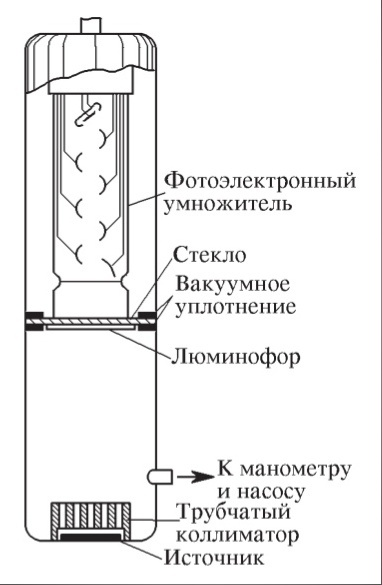
\includegraphics[width=10cm]{img/Sin.jpg}
                \caption{Схема экспериментальной установки}
                \label{fig1}
            \end{figure}
            Установка состоит из цилиндрической камеры, на дне которой находится исследуемый препарат. 
            Камера герметично закрыта стеклянной пластинкой, на которую с внутренней стороны нанесен слой люминофора.\par
            Расстояние между препаратом и люминофором составляет 9 см, так что $\alpha$-частицы не могут достигнуть люминофора при обычном давлении. 
            Определение пробега сводится к измерению зависимости интенсивности счета от давления в камере.
    \newpage

        \subsection{Ход работы}

            В ходе эксперимента была получены зависимость числа зарегистроированных частиц от давления. 
            Результаты представлены в таблицы:
            \begin{table}[h!]
                \centering
                \begin{tabular}{|c|c|}
                \hline
                $\Delta P [\text{мм.рт.ст}]$& Кол-во частиц за 10 сек \\ \hline
                720                 & 3602                    \\ \hline
                660                 & 3439                    \\ \hline
                630                 & 3073                    \\ \hline
                640                 & 3276                    \\ \hline
                620                 & 2893                    \\ \hline
                610                 & 2743                    \\ \hline
                600                 & 2534                    \\ \hline
                590                 & 2344                    \\ \hline
                580                 & 2181                    \\ \hline
                570                 & 2034                    \\ \hline
                560                 & 1761                    \\ \hline
                550                 & 1656                    \\ \hline
                540                 & 1370                    \\ \hline
                530                 & 1124                    \\ \hline
                520                 & 920                     \\ \hline
                510                 & 737                     \\ \hline
                500                 & 541                     \\ \hline
                490                 & 370                     \\ \hline
                480                 & 181                     \\ \hline
                470                 & 170                     \\ \hline
                460                 & 60                      \\ \hline
                450                 & 10                      \\ \hline
                420                 & 3                       \\ \hline
                370                 & 2                       \\ \hline
                330                 & 2                       \\ \hline
                \end{tabular}
            \end{table}\par
            По полученнм даннм был построен график зависимости N(P), затем экспериментальные точки были приближены полиномом 10 степени. 
            От полинома была найдена производная и по ее экстремуму было оперделено среднее давление:
            \begin{equation}
                P_\text{Ср} = 209 [\text{мм.рт.ст}]
            \end{equation}\par
            Участок спада был экстраполирован прямой до пересечения с осью X.
            Таким образом было получено экстраполированное значение давления:
            \begin{equation}
                P_\text{Экстр} = 268 [\text{мм.рт.ст}]
            \end{equation}\par
    \newpage
            
            \begin{figure}[h!]
                \centering
                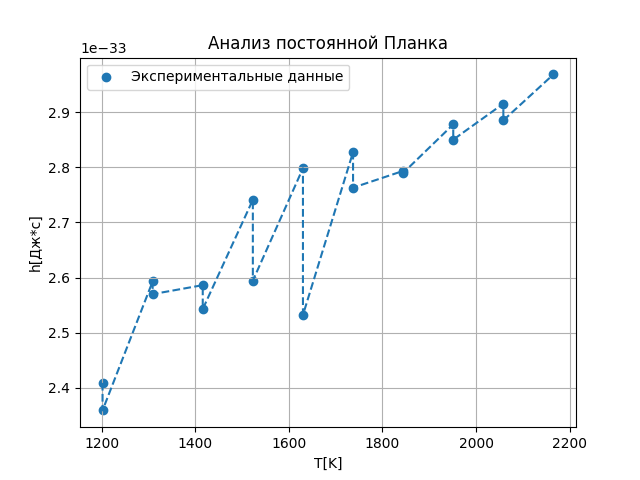
\includegraphics[width=18cm]{img/Graph2.PNG}
                \caption{График зависимоти N(P)}
                \label{graph2}
            \end{figure}\par
            С учетом погрешностей приближения относительную погрешность давления оценим как:
            \begin{equation}
                \delta_P \approx 0.05
            \end{equation}\par
            Значения с учетом погрешностей:
            \begin{equation}
                P_\text{Ср} = 209 \pm 10 [\text{мм.рт.ст}] \hspace{10mm}
                P_\text{Экстр} = 268 \pm 13 [\text{мм.рт.ст}]
            \end{equation}\par
            Расчет длины свободного пробега:
            \begin{equation}
                R_{\text{Ср}} = R \frac{P_0 T_n}{P_n T_0} = 9 \frac{209(15 + 273)}{760 (22 + 273)} = 2.41~ \text{см}
            \end{equation}\par
            \begin{equation}
                R_{\text{Экстр}} = R \frac{P_0 T_n}{P_n T_0} = 9 \frac{268(15 + 273)}{760 (22 + 273)} = 3.10~ \text{см}
            \end{equation}\par
            Значения с учетом погрешностей:
            \begin{equation}
                R_\text{Ср} = 2.41 \pm 0.12 [\text{см}] \hspace{10mm}
                R_\text{Экстр} = 3.10 \pm 0.16 [\text{см}]
            \end{equation}\par
\end{document}